\colorfulheader{computer vision}

\begin{minipage}[t]{0.465\textwidth}
  \begin{itemize}[leftmargin=*]
    \setlength\itemsep{0pt}
    \item \textbf{Computer Vision} is the area of inferring properties given an image. Its pipeline can be simplified as
    \begin{customcenter}[0pt]
        \resizebox{7.5cm}{7.5cm}{
        \begin{tikzpicture}
            \node (cv1) [draw,text centered,text width=7cm,fill=purple!20] {\textbf{Specify Image} \\ \vspace{-6pt}\rule{\textwidth}{1pt} \\ $[\underbrace{\texttt{RGB,CYK}}_{\text{Color Model}}\dots\underbrace{\texttt{PNG,JPG}}_{\text{Compression}}\dots\underbrace{\texttt{uint32,float}}_{\text{Data Type}}\dots]$};
            \node (cv2) [draw,text centered,text width=9.5cm,fill=blue!20,below of=cv1,yshift=-1.1cm] {\textbf{Pre-processing} \\ \vspace{-6pt}\rule{\textwidth}{1pt} \\ $[\underbrace{\text{Resize \textbar\hspace{3pt}Reshape}}_{\text{Aspect Ratio, ROI, etc.}}, \underbrace{\text{Transformations}}_{\text{Rotation, Reflection, etc.}}, \underbrace{\text{RGB To Gray}}_{\text{Mapping, Filtering, etc.}}]$};
            \node (cv3) [draw,text centered, text width=7cm,fill=green!20,below of=cv2,yshift=-2.5cm] {\textbf{Algorithm} \\ \vspace{-6pt}\rule{\textwidth}{1pt} \\ $\underbrace{\text{Transformations}}_{\substack{\text{Convolution} \\ \text{Discrete Fourier Transform} \\ \text{Histograms}}}$ \\ Camera Calibration \textbar\hspace{0pt} Undistorsion \\ Feature Extraction $|$ Segmentation \\ Optical Flow \textbar\hspace{0pt} Tracking \\ $\underbrace{\text{SFM}}_{\substack{\text{Structure} \\ \text{From Motion}}}$ \textbar\hspace{0pt} $\underbrace{\text{SLAM}}_{\substack{\text{Simultaneous} \\ \text{Location And} \\ \text{Mapping}}}$};
            \node (cv4) [draw,text centered,text width=10cm,fill=yellow!20,below of=cv3,yshift=-2.45cm] {\textbf{Post-processing} \\ \vspace{-6pt}\rule{\textwidth}{1pt} \\ $[\text{Some as pre-processing}, \underbrace{\text{Kernels \textbar\hspace{3pt}Matrix Operators}}_{\text{Blurring, Smoothing Sharpening, etc.}}]$};
            \node (cv5) [draw,text centered,fill=red!20,below of=cv4,yshift=-0.5cm] {\textbf{Display $|$ Data Output}};
            \draw [arrow] (cv1) -- node[anchor=south]{} (cv2);
            \draw [arrow] (cv2) -- node[anchor=south]{} (cv3);
            \draw [arrow] (cv3) -- node[anchor=south]{} (cv4);
            \draw [arrow] (cv4) -- node[anchor=south]{} (cv5);
        \end{tikzpicture}
        }
    \end{customcenter}
    \item Important \textbf{kernels} in computer vision
    \begin{customcenter}[-18pt]
      \begin{align*}
          &
          \overbrace{
          \underbrace{
          \frac{1}{9}
          \begin{bmatrix}
          1 & 1 & 1 \\
          1 & 1 & 1 \\
          1 & 1 & 1
          \end{bmatrix}
          }_{\text{Box}}
          \underbrace{
          \frac{1}{16}
          \begin{bmatrix}
          1 & 2 & 1 \\
          2 & 4 & 2 \\
          1 & 2 & 1
          \end{bmatrix}
          }_{\text{Gaussian}}
          }^{\text{Blur}}
          \overbrace{
          \underbrace{
          \begin{bmatrix}
          0 &  1 & 0 \\
          1 & -4 & 1 \\
          0 &  1 & 0 \\
          \end{bmatrix}
          }_{\text{Laplacian}}
          }^{\text{Sharpening}} \\
          &
          \overbrace{
          \underbrace{
          \overbrace{
          \begin{bmatrix}
          -1 & 0 & 1 \\
          -1 & 0 & 1 \\
          -1 & 0 & 1
          \end{bmatrix}
          }^{x}
          \overbrace{
          \begin{bmatrix}
          -1 & -1 & -1 \\
          \text{\textcolor{white}{+}}0 & \text{\textcolor{white}{+}}0 & \text{\textcolor{white}{+}}0 \\
          \text{\textcolor{white}{+}}1 & \text{\textcolor{white}{+}}1 & \text{\textcolor{white}{+}}1
          \end{bmatrix}
          }^{y}
          }_{\text{Prewitt}}
          \underbrace{
          \overbrace{
          \begin{bmatrix}
          -1 & 0 & 1 \\
          -2 & 0 & 2 \\
          -1 & 0 & 1
          \end{bmatrix}
          }^{x}
          \overbrace{
          \begin{bmatrix}
          -1 & -2 & -1 \\
          \text{\textcolor{white}{+}}0 & \text{\textcolor{white}{+}}0 & \text{\textcolor{white}{+}}0 \\
          \text{\textcolor{white}{+}}1 & \text{\textcolor{white}{+}}2 & \text{\textcolor{white}{+}}1
          \end{bmatrix}
          }^{y}
          }_{\text{Sobel}}
          }^{\text{Edge Detection}}
      \end{align*}
    \end{customcenter}
    \vspace{12pt}
    \item Vision uses the \textbf{pinhole camera model}, consisting of \textbf{extrinsic} and \textbf{intrinsic} camera paremeters
    \item Extrinsic values can be encoded in the matrix $\bracketA{\substack{R_{3x3}\;T_{3x1} \\ \\ 0_{1x3}\;\text{\textcolor{white}0}1\text{\textcolor{white}0}}}$. In camera coordinates $R$ represents the \textit{world axes} and $T$ the \textit{world origin}. In \texttt{OpenGL} can be computed via \inlinecode{glm::lookAt()}
    \item Intrinsic values represent the internal parameters of the camera, such as \textit{focal length}, \textit{skew}, and \textit{principal point}. It can be obtained via \textbf{calibration} but in \texttt{OpenGL} represents the \textit{projection matrix} such as \inlinecode{glm::perspective()}
    \item Scale$-$Invariant Feature Transform \textbf{\parenthesis{SIFT}} is a \textbf{feature detection algorithm} invariant to scale and rotation
    \item \textbf{SIFT} is an improvement of \textit{Harris algorithm} (only rotation invariant)
    \item \textbf{Image Registration} is the process of \textbf{matching features} between images. Matching can be done by comparing keypoints and finding \textbf{coresspondences}
    \begin{customcenter}[-3pt]
      \begin{tikzpicture}
        \tikzstyle{appnode}=[draw,minimum height=0.75cm,minimum width=1.5cm,text width=1.5cm,text centered]
        \node[draw,fill=red!40](n1){Image Registration};
        \node[appnode,below of=n1,xshift=-3.70cm](n1a){$\substack{\text{Motion}\\\text{Tracking}}$};
        \node[appnode,below of=n1,xshift=-1.85cm](n1b){$\substack{\text{Object}\\\text{Recognition}}$};
        \node[appnode,below of=n1,xshift=+0.00cm](n1c){$\substack{\text{Optical}\\\text{Flow}\\\text{\tiny{Feature-Based}}}$};
        \node[appnode,below of=n1,xshift=+1.85cm](n1d){$\substack{\text{Depth}\\\text{Estimation}}$};
        \node[appnode,below of=n1,xshift=+3.70cm](n1e){$\substack{\text{Image}\\\text{Stitching}}$};
        \node[draw,xshift=+2.8cm,yshift=0.35cm](n1f){$\substack{\text{Robot}\\\text{Localization}}$};
        \node[draw,xshift=-2.8cm,yshift=0.35cm](n1g){$\substack{\text{Structure}\\\text{From Motion}}$};
        \draw[arrow] (n1) -| (n1a);
        \draw[arrow] (n1) -| (n1b);
        \draw[arrow] (n1) -- (n1c);
        \draw[arrow] (n1) -| (n1d);
        \draw[arrow] (n1) -| (n1e);
        \draw[arrow] (n1.north) |- (n1f.west);
        \draw[arrow] (n1.north) |- (n1g.east);
      \end{tikzpicture}
    \end{customcenter}
    \item RANdom Sample Consensus \textbf{\parenthesis{RANSAC}} is an \textbf{iterative probabilistic} method to \textbf{estimate parameters} of a mathematical model from a set of observed data containing outliers
  \end{itemize}
\end{minipage}
\hspace{10pt}
\begin{minipage}[t]{0.485\textwidth}
  \begin{itemize}[leftmargin=*]
    \setlength\itemsep{0pt}
    \item \textbf{Convolution} is a mathematical operation on \textbf{two functions} $\parenthesisA{f\text{ and }g}$ that \textbf{produces a third function} $\parenthesisA{f*g}$ that expresses \textit{how the shape of one is modified by the other}. Formally,
    \begin{align*}
        \parenthesisA{f*g}\parenthesisA{t} = \int_{-\infty}^{+\infty}f\parenthesisA{\tau}g\parenthesisA{t - \tau}d\tau
    \end{align*}
    \vspace{-10pt}
    \item It can be generalized to $n$ dimensions and in practice the integral can be changed for a summation $\parenthesisA{\sum}$ while the integral limits are defined by the problem's context. The discratization is denoted \textbf{discrete convolution}. For example, a 2D convolution in image processing would be
    \begin{align*}
      \text{Conv2D}\parenthesisA{x,y} = \sum_{i=-\frac{n}{2}}^{\frac{n}{2}}\sum_{j=-\frac{m}{2}}^{\frac{m}{2}}h\parenthesisA{i,j}I\parenthesisA{x - i, y - j}
    \end{align*}
    \vspace{-8pt}
    \begin{customcenter}[0pt]
      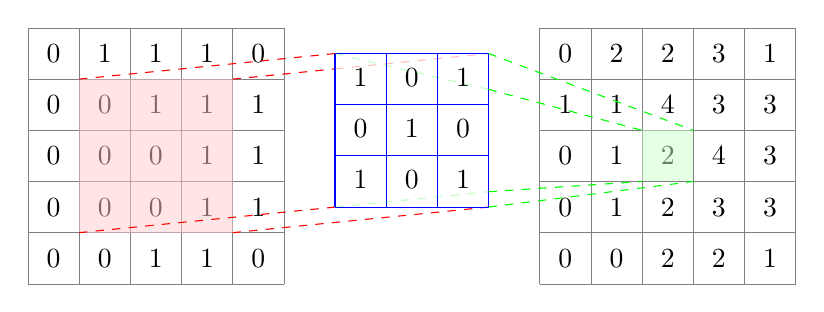
\begin{tikzpicture}
        \begin{scope}[scale=0.65]
          \draw[step=1cm,gray,very thin] (0,0) grid (5,5);
          \node[] at (0.5,0.5){0};
          \node[] at (1.5,0.5){0};
          \node[] at (2.5,0.5){1};
          \node[] at (3.5,0.5){1};
          \node[] at (4.5,0.5){0};
          \node[] at (0.5,1.5){0};
          \node[] at (1.5,1.5){0};
          \node[] at (2.5,1.5){0};
          \node[] at (3.5,1.5){1};
          \node[] at (4.5,1.5){1};
          \node[] at (0.5,2.5){0};
          \node[] at (1.5,2.5){0};
          \node[] at (2.5,2.5){0};
          \node[] at (3.5,2.5){1};
          \node[] at (4.5,2.5){1};
          \node[] at (0.5,3.5){0};
          \node[] at (1.5,3.5){0};
          \node[] at (2.5,3.5){1};
          \node[] at (3.5,3.5){1};
          \node[] at (4.5,3.5){1};
          \node[] at (0.5,4.5){0};
          \node[] at (1.5,4.5){1};
          \node[] at (2.5,4.5){1};
          \node[] at (3.5,4.5){1};
          \node[] at (4.5,4.5){0};
          \fill[red!20!white,semitransparent] (1,1) rectangle (4,4);
          \draw[red,dashed] (1,1) -- (6,1.5);
          \draw[red,dashed] (4,1) -- (9,1.5);
          \draw[red,dashed] (1,4) -- (6,4.5);
          \draw[red,dashed] (4,4) -- (6,4.2);
          \draw[red,dashed,nearly transparent] (6,4.2) -- (9,4.5);
          \draw[blue,xshift=5cm,yshift=0.5cm] (1,1) grid (4,4);
          \node[xshift=3.25cm,yshift=0.35cm] at (1.5,1.5){1};
          \node[xshift=3.25cm,yshift=0.35cm] at (2.5,1.5){0};
          \node[xshift=3.25cm,yshift=0.35cm] at (3.5,1.5){1};
          \node[xshift=3.25cm,yshift=0.35cm] at (1.5,2.5){0};
          \node[xshift=3.25cm,yshift=0.35cm] at (2.5,2.5){1};
          \node[xshift=3.25cm,yshift=0.35cm] at (3.5,2.5){0};
          \node[xshift=3.25cm,yshift=0.35cm] at (1.5,3.5){1};
          \node[xshift=3.25cm,yshift=0.35cm] at (2.5,3.5){0};
          \node[xshift=3.25cm,yshift=0.35cm] at (3.5,3.5){1};
          \draw[step=1cm,gray,very thin,xshift=10cm] (0,0) grid (5,5);
          \node[xshift=6.5cm] at (0.5,0.5){0};
          \node[xshift=6.5cm] at (1.5,0.5){0};
          \node[xshift=6.5cm] at (2.5,0.5){2};
          \node[xshift=6.5cm] at (3.5,0.5){2};
          \node[xshift=6.5cm] at (4.5,0.5){1};
          \node[xshift=6.5cm] at (0.5,1.5){0};
          \node[xshift=6.5cm] at (1.5,1.5){1};
          \node[xshift=6.5cm] at (2.5,1.5){2};
          \node[xshift=6.5cm] at (3.5,1.5){3};
          \node[xshift=6.5cm] at (4.5,1.5){3};
          \node[xshift=6.5cm] at (0.5,2.5){0};
          \node[xshift=6.5cm] at (1.5,2.5){1};
          \node[xshift=6.5cm] at (2.5,2.5){2};
          \fill[green!20!white,semitransparent,xshift=10cm] (2,2) rectangle (3,3);
          \node[xshift=6.5cm] at (3.5,2.5){4};
          \node[xshift=6.5cm] at (4.5,2.5){3};
          \node[xshift=6.5cm] at (0.5,3.5){1};
          \node[xshift=6.5cm] at (1.5,3.5){1};
          \node[xshift=6.5cm] at (2.5,3.5){4};
          \node[xshift=6.5cm] at (3.5,3.5){3};
          \node[xshift=6.5cm] at (4.5,3.5){3};
          \node[xshift=6.5cm] at (0.5,4.5){0};
          \node[xshift=6.5cm] at (1.5,4.5){2};
          \node[xshift=6.5cm] at (2.5,4.5){2};
          \node[xshift=6.5cm] at (3.5,4.5){3};
          \node[xshift=6.5cm] at (4.5,4.5){1};
          \draw[green,dashed] (9,1.5) -- (13,2);
          \draw[green,dashed] (9,4.5) -- (13,3);
          \draw[green,dashed,nearly transparent] (6,1.5) -- (9,1.8);
          \draw[green,dashed] (9,1.8) -- (12,2);
          \draw[green,dashed,nearly transparent] (6,4.5) -- (9,3.8);
          \draw[green,dashed] (9,3.8) -- (12,3);
        \end{scope}
      \end{tikzpicture}
      \begin{lstlisting}[frame=single]
        bool outOfBounds(int n, int m, int w, int h)
        {
          return (n < 0 || n > h - 1 || m < 0 || m > w - 1);
        }
        typedef vector<vector<int>> vvint;
        vvint convolution2D(const vvint & M, const vvint & K)
        {
          vvint convolution;
          int height = M.size();
          int width = M[0].size();
          int n2 = K.size() / 2;
          int m2 = K[0].size() / 2;
          convolution.resize(M.size());
          for (int n = 0; n < height; n++)
          {
            convolution[n].resize(width);
            for (int m = 0; m < width; m++)
            {
              int sum = 0;
              for (int i = -n2; i <= n2; i++) 
              {
                for (int j = -m2; j <= m2; j++) 
                {
                  // Clamp result in bounds
                  if (!outOfBounds(n - i, m - j, width, height))
                  {
                    sum += (K[i + n2][j + m2] * M[n - i][m - j]);
                  }
                }
              }
              convolution[n][m] = sum;
            }
          }
          return convolution;
        }
      \end{lstlisting}
    \end{customcenter}
    \item \textbf{Optical flow} is the technique of \textbf{understanding the motion of a scene}. Can be \underline{\textit{freature-based}}, where one finds features between two frames, or \underline{\textit{dense}}, where correspondences between frames applies to all pixels (one algorithm is energy minimization Lucas-Kanade)
  \end{itemize}
\end{minipage}